\documentclass{article}
\usepackage{amsmath}
\usepackage{tikz}
\usetikzlibrary{matrix, shapes.geometric}

\begin{document}

\begin{figure}[h]
    \centering
    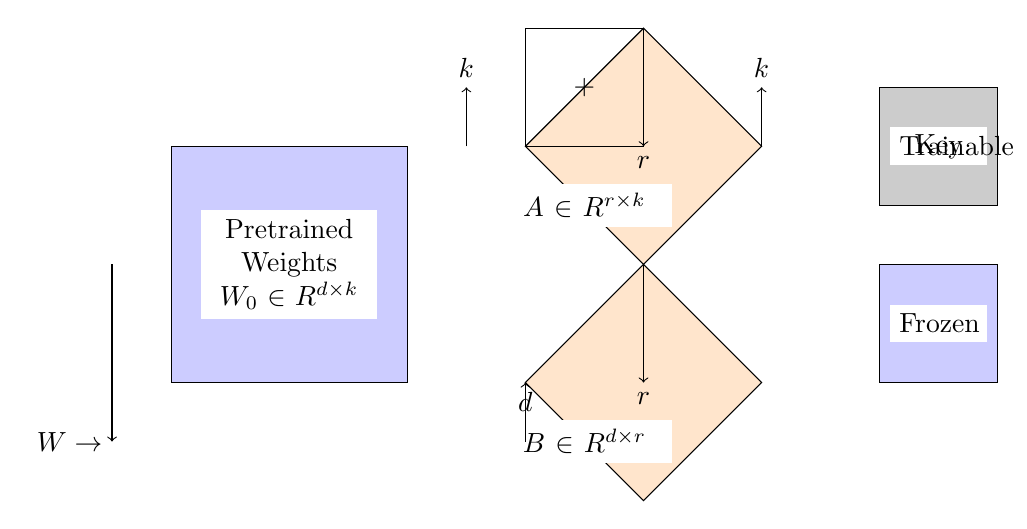
\begin{tikzpicture}[scale=1.5]
        % Draw the rectangle for the pretrained weights
        \draw[fill=blue!20] (0,0) rectangle (2,2) node[midway, fill=white, text width=2cm, align=center] {Pretrained\\Weights\\$W_0 \in \mathbb{R}^{d \times k}$};
        
        % Draw the parallelogram for B
        \draw[fill=orange!20] (3,0) -- (4,1) -- (5,0) -- (4,-1) -- cycle node[midway, fill=white, text width=2cm, align=center] {$B \in \mathbb{R}^{d \times r}$};
        
        % Draw the parallelogram for A
        \draw[fill=orange!20] (3,2) -- (4,3) -- (5,2) -- (4,1) -- cycle node[midway, fill=white, text width=2cm, align=center] {$A \in \mathbb{R}^{r \times k}$};
        
        % Draw the summation symbol
        \draw (3,2) -- (3,3) -- (4,3) -- (4,2) -- cycle;
        \node at (3.5, 2.5) {$+$};
        
        % Draw the arrows and labels
        \draw[->] (-0.5, 1) -- (-0.5, -0.5) node[left] {$W \rightarrow$};
        \draw[->] (2.5, 2) -- (2.5, 2.5) node[above] {$k$};
        \draw[->] (5, 2) -- (5, 2.5) node[above] {$k$};
        \draw[->] (3, -0.5) -- (3, 0) node[below] {$d$};
        \draw[->] (4, 1) -- (4, 0) node[below] {$r$};
        \draw[->] (4, 3) -- (4, 2) node[below] {$r$};
        
        % Draw the key box
        \draw[fill=blue!20] (6,0) rectangle (7,1) node[midway, fill=white, text width=1cm, align=center] {Frozen};
        \draw[fill=black!20] (6,1.5) rectangle (7,2.5) node[midway, fill=white, text width=1cm, align=center] {Trainable};
        \node at (6.5, 2) {Key};
    \end{tikzpicture}
\end{figure}

\textbf{Caption:} A visual representation of the training scheme for LoRA. The update of $W$ is given by $W_0 + BA$ where $B$ and $A$ are of a particular low-rank form.

\end{document}